\chapter{Implemented Features}

In this chapter we present the implementation details of some non-trivial modules.

\section{Granting unique request IDs}

A request must be different for each request. Only this guarantees that we will be able to say if a request is retransmitted, or it's a new one. A common method is to split the request identification in two parts: the client ID and sequential number. As far as assigning sequential number is trivial, method providing unique client ID's must be carefully chosen, especially taking under consideration the crash-recovery model.

The client ID has to be unique for two different clients. To guarantee this, replicas must be responsible for granting ID's to clients, because a client has no knowledge of other client's ID.

\paragraphNewline{Based on number of replicas}
Each replica can grant numbers incremented by number of replicas, starting from ID of local replica. For example, if we have three replicas, replica with ID 0 can grant numbers 0, 3, 6, 9, ... and replica with ID 2 can grant 2, 5, 8, ... . It guarantees that two different replicas will not grant the same ID. This solution works with crash-stop and crash-recovery with stable storage. This will not work when replica can recover from crash without stable storage, because it doesn't now what was the last granted ID.

\paragraphNewline{Time based}
This is different approach -- we use system time as the source if unique numbers. To each client ID we are adding also information when replica was started (in milliseconds).

If replica started at time $t$, it will grant ID's $(t + localId)$, $(t + localId + n)$, $(t + localId + 2n)$...

It assumes that local system timer is not set back into past and also that replica will not recover in the same millisecond. If these assumptions are fulfilled, then they guarantee unique IDs in crash-recovery model without stable storage. This approach is currently default in our library.

\paragraphNewline{View based}
Because time based assumptions sometimes cannot be guaranteed, another approach for crash-recovery model may be considered. Instead of adding information about start time, we can add current view number. In each view, there is exactly one leader -- so after the prepare phase this replica can grant clients IDs as pair (view, sequence number). Two different replicas cannot start the same view.
Also we have to guarantee that only leader replica after prepare phase can grant new client IDs.

This approach will also work by using the Epoch numbers -- if a leader crashes, the view must be increased by his recovery.


\section{Catch-up}
\label{sec:catch_up}

\paragraphNewline{Motivation}

Paxos must guarantee that every valid replica will eventually decide. Most papers about Paxos state that if a replica notices lack of activity for some instance, it will send new proposal and eventually decide. But by using view for all instances, this would mean often view changes -- and this contradicts performance.

Therefore a different approach is used by us: as we know that if the leader is correct, it will decide, otherwise a new leader will be elected. If the leader is correct, and no activity about an instance is noticed, that means the value is already decided and the replica is in the minority that does not know  about the decision.

In such case, instead of forcing a new proposal, we use the Catch-up module.
The Catch-up has to download all missing decisions. This solution is faster than new ballot if the instance is already decided and it does not need a view change.

\paragraphNewline{Recovery}

This module is also used by recovering the replica -- as a tool for downloading all decided instances up to required state.

But there is one drawback -- for the recovery one needs to know also instances yet undecided.  However, if the system is operational, after a short time all required instances will be decided. If the system is not operational the recovery cannot converge. So downloading only decided instances is correct, but may cause small delay by recovering

\subsection{Log-based vs state-based recovery}
\label{subsec:log_based_state_based_recovery}
A replica can catch-up either by copying the missing decisions or by a combination of transferring the state plus the most recent decisions.

In the rest of this paper \emph{log-based recovery} refers to the first option while \emph{state-based recovery} refers to the second option.

The method that is fastest will depend on the particular characteristics of the system:

\begin{description}
  \item[Size of the state] For services with large states, it's better to avoid transferring the state as much as possible. On the other hand, if the service state is small, transferring it might be better. In the extreme case, the service state is of a similar size or smaller than the individual commands. In this case, it would always be better to transfer the state.

  \item[Execution overhead] Executing commands takes some processing time which is not required when transferring the state. Therefore, even if the service state is bigger than the corresponding commands, it might be faster to transfer the state.

  \item[Bandwidth available] With limited bandwidth, the fastest  method will likely be the one that transfers less data. Otherwise, the execution overhead will likely be the dominant factor.
\end{description}

\paragraph{State-based recovery time}

State-base recovery has the following steps:

\begin{table}[H]
  \footnotesize
  \begin{center}
    \begin{tabular}{ll}
      Serialisation               & state is transformed into a sequence of bytes \\
      Transfer                    & size is sent via network \\
      Deserialization             & state is rebuilt at destination \\
      &\\
      Residual log-based-recovery & recovery from snapshot process is made \\
    \end{tabular}
  \end{center}
  \vspace{-1em}
\end{table}

The first three tasks may be done concurrently. Assuming that the fourth task is comparatively fast, we can consider that the total recovery time is the maximum time it takes to do each of the first three tasks.

\paragraph{Log-based recovery time}

Log-based recovery consists only on sending the commands and executing them at the replica. Once again, sending and executing can be done concurrently, so the total duration is the max of the time it takes to transfer all the updates or to execute them.

\subsection{Conditions for starting and finishing the catch-up}
\label{subsec:conditions_for_starting_and_finishing_the_catch_up}
Many possible rationales may be used as indicator, when the process should begin the catch-up. Also conditions needed for the stop process are a significant issue.

\paragraph*{Starting catch-up}
Activating the mechanism should not happen too early, that is when Paxos itself is still able to take the decision -- target of catch-up is to complement decisions missing due to packet loss. On the other hand late initiating leads to delaying command execution, and thus significant performance loss.

Most common events used to initialise the algorithm are:
\begin{itemize}
  \item No traffic for the ballot during a particular period of time (\textsc{timeout})
  \item An instance with higher ID (i.e. newer instance) has already been decided (\textsc{higher instance decided})
  \item Instance with ID higher than $\alpha$ has been started, and the implementation ensures that only instances up to $\alpha$ are started as $\alpha-ws$ stays undecided (\textsc{window})
  \item Activate periodically the mechanism (\textsc{periodical})
\end{itemize}

These methods let the replica suspect, that a locally undecided instance has already been decided, so it's log state is not up to date. It's good to use more than one of them, as each method is sensitive for a particular scenario, perhaps performing bad otherwise.

Simplest, but not efficient for most uses is the \textsc{periodical} method -- it guarantees that from time to time the replica will be up to date.
Too often used may cause bandwidth and processor consumption, too rarely -- having old state for unacceptably long time.

The \textsc{timeout} event is caused either if problems with network occur, or if the \accept messages were lost -- otherwise current leader and other replicas would generate traffic for the ballot. The replica should try to learn the state of voting in such case, otherwise as long as no new proposal will arise, the replica will have old state.

\textsc{higher instance decided} means that a later started voting already finished. We may assume the previous voting took similar amount of time -- that is, it should be already finished. Message loss or varying latency can also cause the situation that a newer consensus is decided as the older is still in progress. To avoid this situation the method may be extended to this: if the number of newer decided instances exceeds a constant value, then the catch-up should be initiated.

The method, as well as the earlier described, may be used in case when operations on state machine require long processing. Risk of loosing small bandwidth for catch-up may be small enough compared to earlier arrival time of resource-consuming task.

The \textsc{window} method is only one guaranteed, because of it's assumption: the algorithm uses window of maximum size $ws$. If the condition that all decisions outside the window must be decided is violated on one replica, it means that other replicas, at least current leader, already decided the instance. This means no new messages concerning the ballot will emerge, and catch-up is necessary.

A different problem is when a replica doesn't know that the instance already exists (for example, a short-time netsplit or bad luck caused all messages for the replica to be dropped). In this case, the catch-up should be started as well. 
Either periodic requests must be sent, or additional information must be acquired. It should be emphasised, that as any newer ballot starts, the replica is informed about the existence of missing instance. 

Although this is not critical, it prevents state machine from executing the command until new instance emerges. That means performance loss, as the old command must be caught-up and executed before the new.

In our system, replica is notified about highest instance id from \alive message from leader. The leader is attaching this number to every \alive message sent. This guarantees that every replica learns what instances already exists within failure detector timeout.

\paragraph*{Stopping catch-up} As the algorithm runs, the state of Paxos may not be stable, i.e. new ballots may start. Therefore selecting the moment when catch-up should be deactivated is not trivial.

One method is to calculate conditions a priori (for example the IDs of missing instances), and continue the process as long as needed. But this can easily lead to a constant switching on and off the catch-up -- voting for new instances may be faster than catching up, so as the predefined conditions are met, new event already caused catch-up activation.

The better solution is to determine dynamically if catch-up is still needed. A method, that seems most convenient for that is checking, if all instances outside the window are already decided. Stopping earlier is bad, as we know that at least the current leader must have decided for the missing instances, and that means we will not get the value via Paxos algorithm.

Finishing the catch-up process later, that is requiring any messages in the window to be decided is also not a good solution -- unless we have some additional knowledge that the instance has already been decided (for example, leader's last uncommitted instance ID is sent in \propose or \alive messages).

Problem arises, if there really were decided instances inside the window. If there are no new ballots, arrival time of these requests will be delayed. In our opinion, the problem is not that severe, especially if window size does not exceed reasonable size.

\subsection{Transport protocol}
\label{subsec:transport_protocole}
As totally separate from Paxos, the catch-up may use different transport protocol than the consensus algorithm.
Choice of transport layer must take into account characteristics of this mechanism as well.

Both TCP and UDP may be used -- both having their pros and cons, presented in table below

\begin{center}
\small
\begin{tabular}{>{\raggedleft\hspace{0pt}}m{0.47\textwidth}m{0.47\textwidth}}

\multicolumn{1}{c}{ \textbf{TCP} }& \multicolumn{1}{c}{ \textbf{UDP} } \\ 
automatic retransmission guaranteed by protocol &
                                retransmission must be implemented manually \\ 
flow control provided by protocol & no flow control, it \emph{is} easy to congest network \\
big messages automatically fragmented, mer\-ged and managed &
                                splitting and handling big messages must be~self implemented \vspace{0.5em} \\

request cannot be changed at retransmission &
                                request can be changed each retransmission \\
default retransmission time & custom retransmission time \\
another message may be sent once the previous was delivered &
                                new datagram may be sent anytime, no matter if the previous reached the target \\

\end{tabular}
\end{center}

When catch-up is needed,  our network must have (probably high) message loss. That means catch-up messages may also get easily lost.

We have noticed, that it is more efficient to use UDP for all smaller messages -- if the package gets lost, we're retransmitting it with updated query. Sometimes even twice retransmitted UDP message is faster than one TCP. In TCP, the timeout for ACK message grows automatically - and that may cause big delays. During experiments, with 30\% message loss, transmitting a message using TCP smaller than UDP-datagram size took even more than 4 seconds to reach the other side.

In UDP, single message delay or loss does not block communication to the replica -- but in TCP does.
In this case no new catch-up query may be sent to this replica, as long as the previous will be processed. The request cannot of course be changed. It means that once we got the response, core protocol may have already missed another instances to catch-up.

\subsection{Requirements}
\label{subsec:catch_up_requirements}
The speed and resource consumption must be correctly balanced.

In theory, catching-up can be delayed any finite time. On the other hand, it is important for view changes and for bounding the size of the log. A view change will take longer if the new leader is missing many requests. Since during a view change no new requests are being satisfied, we need to keep its length as short as possible. Additionally, if a replica doesn't know instance $i$, it cannot execute any request higher than $i-1$. This also means that it cannot remove entries from the log.

In practical approach most significant requirements for catch-up are: good performance and small resource usage. For sure catching up should not slow down the core protocol.
Good performance demand has one main reason: arrival time of the tasks for state machine is dependent on being up to date. If catch-up would get information too late, the state machine would get long list of, possibly high CPU-consuming, tasks at once, instead of doing them in spare time before.

Therefore, it is desirable to catch-up as often as possible, but without slowing down the service significantly.

It should be noticed, that only the followers will have to catch-up, since the primary learns of all previous decisions on a view change and then is the one proposing new values and leading the protocol.

\subsection{Catch-up algorithm}
\label{subsec:catch_up_algorithm}
The catch-up algorithm should contact other replicas and copy the decisions that are not known. Question when this should be done is discussed in section \ref{subsec:conditions_for_starting_and_finishing_the_catch_up}. Here the main idea of JPaxos catch-up algorithm is presented.

To activate the catch-up, we use \textsc{window} and \textsc{periodical} methods (see \ref{subsec:conditions_for_starting_and_finishing_the_catch_up}).

This ensures that the replica will catch-up eventually, even if there are no new requests, and that a replica never stays too much behind the others, at most $\alpha$.

There are three messages, that may be sent during the algorithm: \catchUpQuery, \catchUpResponse and \catchUpSnapshot.
\begin{description}
 \item[\normalfont\catchUpQuery] Request for missing instances. Carries list of missing ID's and may have one of the two flags set: first flag indicates if this was a periodical catch-up, second -- if we want to get last snapshot, not missing log fragment.
 \item[\normalfont\catchUpResponse] Response sent for every received request. Has list of decided instances for requested numbers. The list may be empty. This message may have two flags: either if the query had periodical flag set, or indicator that the replica doesn't have old enough log, and state transfer is the only possibility.
 \item[\normalfont\catchUpSnapshot] If another replica asked for our last snapshot, this message is sent. It contains only responders last snapshot.
\end{description}

The list describing missing instances is constructed quite simple: it contains all undecided instance numbers plus the (highestID+1) as the first instance replica has no knowledge about. The responder sends therefore all decided from the list + all decided instances higher or equal than the additional number.

In order to make the messages smaller, a trick has been used: the list contains of two lists. One called range list and the other instance list.
Range list contains intervals we miss, while instance list -- single numbers. For example, if we would miss instances 1,2,4,6,7,8,9,11, and the highest instance we know is 12 (state decided) our lists would look like:
\begin{quote}
$[\langle1,2\rangle; \langle6,9\rangle]; [4,11,13]$
\end{quote} 
Notice the number 13 -- it's the first we have no idea of existing, as mentioned above.

Catch-up works as follows:

\begin{algorithmic}[1]
  \REPEAT
    \STATE \label{alg_1_a} Choosing target replica
    \STATE Creating list of missing instances
    \STATE Send a \catchUpQuery
    \STATE \label{alg_1_b} Wait for timeout or for response
  \UNTIL{\label{alg_1_c} catch-up succeeds}
  
  \vspace{1em}
  
  \STATE \textbf{upon} receiving \catchUpQuery \textit{query}
    \IF{\textit{query} has snapshot flag set}
      \STATE Get last snapshot
      \STATE Prepare \catchUpSnapshot message
      \STATE Send the message
    \ELSIF{requested instances already not in log}
      \STATE Send \catchUpResponse with \textit{snapshot} flag
    \ELSE
      \STATE Gather all decided instances
      \STATE Send \catchUpResponse
    \ENDIF

  \vspace{1em}
  \STATE \textbf{upon} receiving \catchUpResponse \textit{response}
    \IF{\textit{response} has \textit{snapshot} flag set}
      \STATE Prepare \catchUpQuery with snapshot flag
      \STATE Send the query
    \ELSE
      \STATE Merge received log (if any)
      \STATE Wake up the Catch-up loop (line \ref{alg_1_b})
    \ENDIF
  
  \vspace{1em}
  \STATE \textbf{upon} receiving \catchUpSnapshot \textit{snapshot}
  \STATE Check if \textit{snapshot} is newer than current one
  \STATE Replace the current snapshot with \textit{snapshot}
  \STATE Truncate logs (to stop catch-up)
  \STATE Wake up the Catch-up loop (line \ref{alg_1_b})

\end{algorithmic}

\vspace{1em}

In line \ref{alg_1_a} a best replica is chosen. We've implemented it as follows: a rating for each replica is kept. When sending a message, the rating decreases; when receiving response - rises. If an empty response is received (except for \textsc{periodic} mode), we request asking the leader next time. Best replica for us is a follower with highest positive rating, or the leader if all followers have negative rating.

Magic line \ref{alg_1_c} executes a predicate checking if the catch-up shall finish (see \ref{subsec:conditions_for_starting_and_finishing_the_catch_up}).

\section{Snapshotting}
\label{sec:snapshotting}
As presented before, the support of storing and transmitting state of replicated machine is very useful and important part of a replica. In practical systems it is necessary -- it allows log truncating, faster recovery and catch-up.

\subsection{When to snapshot}
\label{subsec:when_to_snapshot}
Snapshots are needed in two cases: to enable catch-up and recovery, and to truncate the log. For both uses there is a different ``best moment'' for making snapshot.

As for recovery, we get best recovery result if the snapshot would be done every executed order.
This, of course, is not the solution. It would completely decrease the throughput - snapshot creation is for sure resource-consuming.

For the catch-up the moment when another replica requests snapshot is the best for creating one. However, we should not demand creating snapshot when we want to, so it's better to rely on the service programmer.

For truncating the log snapshot should just be created periodically, without any additional requirements.

Therefore we assume the snapshot should be made when the cost of catch-up from log becomes bigger than cost of catch-up from snapshot.

Please notice, that catch-up time also includes time of state/log transfer.

\subsection{Replica vs state machine responsibility}
\label{subsec:replica_vs_state_machine_responsibility}
There are two approaches to the problem who is in charge with snapshot creation. Either the replica issues a snapshot, or the state machine chooses appropriate moment and forwards the state to replica.

Embedding this functionality into the replica will surely provide more secure work (state machine may simply not deliver the snapshots, what means forever growing log). It is easier for replica to measure size of the messages that should be transferred in order to catch-up (or recover).

However, the replica does not now anything about state machine. We can also assume, that the service is not aware of network conditions. Therefore choosing the proper moment (when cost of log-based catch-up becomes more expensive than state-based catch-up) is impossible for both. It is clearly visible, that state machine is better informed - it knows not only the size of requests, but also may estimate size of it's current state and resources needed to execute all commands from log.

The latter is most significant difference: replica has no idea how long the log execution from previous snapshot would take. It seems possible to estimate this: measuring time between request and replay might solve the problem. But such estimate can give mistaken result, especially in multi-process environment. If another process is consuming CPU, or the replica waits a long time for granting some resources (like access to a file or even a printer), the estimate surely will not reflect real value.

Table below presents in compact way state of knowledge needed to select best moment for next snapshot:
\begin{center}
% use packages: array
\small
\begin{tabular}{r|c|c|}
\cline{2-3}
 & State machine & Replica \\ \hline 
\multicolumn{1}{|r|}{Size of requests} & known & known \\ \hline
\multicolumn{1}{|r|}{Size of state } & known & estimate \\ \hline
\multicolumn{1}{|r|}{Log execution time} & good estimate & poor estimate \\ \hline
\multicolumn{1}{|r|}{Time for sending message} & unknown & estimate \\ \hline
%\multicolumn{1}{|r|}{ × } & × & × \\ \hline
\end{tabular}
\end{center}

\subsection{Our approach to snapshotting}
\label{subsec:our_approach_to_snapshotting}
Snapshotting, as described above, may be done in a variety of ways. Also how often the snapshots are made depends on implementation. Here we give main clues how the snapshotting is implemented.

The decision who orders a snapshot creation has been left to the future user of the library. To achieve this, some assumptions has been taken -- mainly
concerning architecture of the service.

The service must implement three methods: \texttt{askForSnapshot}, \texttt{forceSnapshot} and \texttt{up\-date\-To\-Snap\-shot}. Also it is required to implement adding and removing snapshot listeners -- objects that implement \texttt{onSnapshotMade} function. When a snapshot is made on the state machine, method \texttt{onSnapshotMade} with the snapshot as parameter must be called on all snapshot listeners.

Replica measures size of the log after every n-th instance, and calculates average size of the snapshot basing on previous ones. By every log measurement a ratio is calculated: $\frac{ \text{log\_size} }{ \text{snapshot\_estimate} }$. As the ratio exceeds one constant, method \texttt{askForSnapshot} is called. After another constant \texttt{forceSnapshot} is executed.

There are several approaches possible on who decides proper time for the snapshot:
\begin{description} 
 \item[State machine only] -- service ignores the functions \texttt{askForSnapshot} and \texttt{forceSnapshot} and does the snapshot on its will.
 \item[Using replica calls as hints] -- service takes under consideration \texttt{askForSnapshot} and \texttt{fo\-rce\-Snapshot} functions, but decides itself when to do snapshot
 \item[Balanced responsibility] -- service uses both \texttt{askForSnapshot} and \texttt{forceSnapshot}; the first as a hint, the latter treats as an order
 \item[Replica only] -- each time \texttt{askForSnapshot} is called, the state machine does snapshot
\end{description}

Snapshotting requires also additional data exchanged between replica and service: the state machine must know the request number, in order to let snapshot identification in replica. For example, if the snapshotting would be done completely on service's side, how would the replica know after which command the snapshot was taken.


\section{Batching}
\label{sec:batching}
Batching means using the same consensus instance to order several requests.

This optimisation does not need any changes to the Paxos algorithm, only requires that requests from one instance can be ordered deterministically by replica, so that replicas know the order in which they should execute the requests. That is no problem, as a byte stream is already ordered -- so each replica will decode the requests the same way.

To achieve multiple requests in the same instance an additional activity must be taken up by proposer and later, by replica, just before execution.

The proposer needs to ``stick'' together the requests, and from that moment on they are treated as one. The other part, dividing it again into requests, should be done after the decision has been taken.
\begin{figure*}[h]
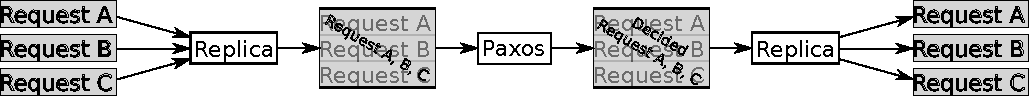
\includegraphics[keepaspectratio, width=\textwidth]{features/batching.pdf}
\end{figure*}

As the count of concurrent instances is bounded (see subsection \ref{subsec:concurrent_instances}), without batching every client needs to wait for his own instance. With batching many client requests may be ``packed'' in one instance. That, on one side, increases the throughput and decreases the delay.
On the other side, message size is getting bigger -- and that means slower voting.

Here arises a question: how many requests to batch? One boundary is quite obvious -- serialized message should not be bigger than transport protocol frame size. As for UDP the size is about 65kB, but for TCP stays unbounded.

From the benchmarks %TODO: referenc on nuno (?)
we can see that best performance and latency is achieved as the batching size is set to the minimal size when all available bandwidth is used.

Another problem concerns the proposer: should there be a lower limit of requests in one instance? Doing so we require waiting for new clients to come. Not waiting means sometimes severe throughput loss.

If we had a single request only, just waiting for an other would cause endless waiting. So a timeout is needed here.

If we decide not to wait at all -- we're packing all the proposer got until now into a single request (if it fits, of course). Such approach guarantees good behaviour if the system state is not changing -- under load, usually we're unable to pack all requests we got, while with small amount of requests no delay by packing decreases the latency.

Both batching size and the timeout for gathering requests in batch is configurable in our library.

\section{Service Proxy}
\label{sec:serviceProxy}

Some operation on service require proper arguments. Should a service be responsible for that? Batching causes that the snapshot can be made after full instances, and not after each request. Should a service take care  for that?

This is not desired. We want to provide as much transparency as possible, without forcing the service to remember redundant data.

\texttt{ServiceProxy} is a module that translates JPaxos instances to Service requests and takes care for all the requirements concerning snapshotting. From Replica side, interaction with the Service through \texttt{ServiceProxy} is instance-oriented and convenient. From Service side, the interaction with clients is as transparent as possible.

To achieve this the \texttt{ServiceProxy} keeps list of responses for all requests from the previous snapshot as well as information required later to restore proper request sequential number from a snapshot.
As the replica provides a snapshot, this module adds to the snapshot required data.

Overhead caused by this proxy should be smaller than the difference in speed of the service if the service were to be aware of instances. The difference is size of the snapshot depends on the state size, but usually the state is much bigger than a few responses required to provide transparency.

Of course, this does not release the service from responsibility of providing valid snapshots. The service still must provide corresponding request sequential number for the snapshot it creates.
